\chapter{Срыв праздника и политический кризис}

Сегодня я вам подробно расскажу про один забавный политический кризис Римской республики. Который как-то совсем потерялся на фоне остальных событий и в истории остался в качестве анекдота про "жену Цезаря, которая должна быть вне подозрений". А между тем интереснейшее событие. На дворе конец 62г до н.э, наступает канун праздника Доброй Богини. За год до этого патрицианская аристократия разгромила Заговор Катилины, где, по слухам, Цезарь с Крассом пытались чужими руками отодвинуть патрициев от власти, но только укрепили их позиции. Помпей недавно вернулся из своих азиатских походов, и теперь ждет когда Сенат ратифицирует его решения в завоеванных территориях и расплатится с его солдатами. А Красс ждет когда ему дадут возможность хорошенько пограбить на Востоке. Цезарь же недавно стал Великим Понтификом Рима, а потом, после претуры, готовится уехать в Испанию Дальнюю в качестве наместника. Всё вроде хорошо, Сенат силен как никогда, все попытки подорвать его позиции терпят крах... ну а дальше давайте по порядку.

\begin{figure}[h!tb]
	\centering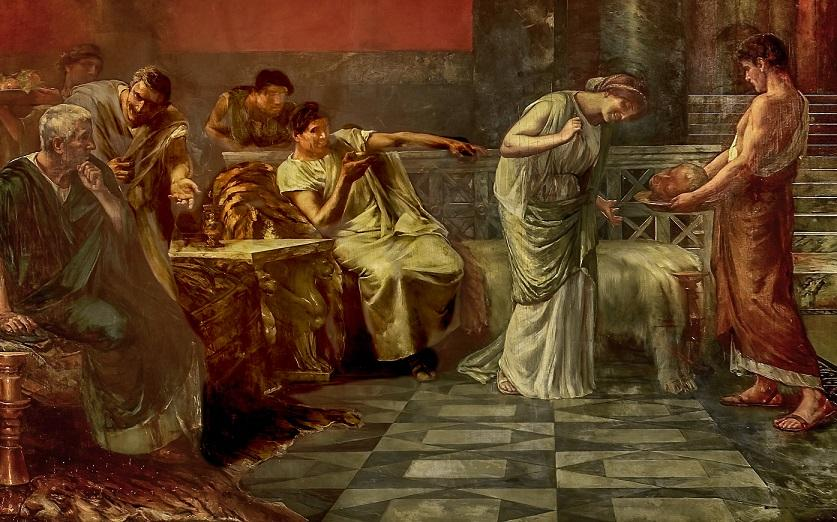
\includegraphics[scale=0.5]{holiday/1593524621164876195.png}
	\label{fig:holid1} % Unique label used for referencing the figure in-text
	%\addcontentsline{toc}{figure}{Figure \ref{fig:placeholder}} % Uncomment to add the figure to the table of contents
	\caption{Подааарочки!!	}
\end{figure}

Праздник Доброй Богини (Весты) это очень сакральное и важное для римлян таинство. В декабре в доме одного из патрициев собираются все знатные матроны Рима и мутят некие ритуальные процедуры, восхваляя свою покровительницу и всё такое. По сути, собирается вся женская часть политической элиты государства. На время праздника сам патриций, все слуги, мужчины, животные и рабы должны покинуть дом и до рассвета там не появляться. А жена хозяина дома становится хозяйкой мероприятия. Сами обряды проводят весталки, священные девственницы, которых в Риме почитали практически на уровне живых богинь. Они, например, могли миловать приговоренных к казни, а за любое оскорбление их достоинства можно было схлопотать смертную казнь без особых разбирательств. И только после того как праздник закончится успешно, весталки там перетрут с богами и скажут что те довольны — в Республике наступает зима. В этом году принимать столь важное мероприятие выпало Гаю Юлию Цезарю. Он, на минуточку, Великий Понтифик города, тоесть глава всего римского жречества, и эта должность пожизненная. А его жена, соответственно, рулит вышеописанным таинством. Всё ОЧЕНЬ серьезно, короче, это вам не вписка какая, а крайне важное мероприятие.


И вот начинается праздник, проходят какие-то ритуалы, вся хурма. А потом ВНЕЗАПНО служанка обнаруживает, что одна из женщин, которые пришли на мероприятие это никакая не женщина, а закутанный в женские шмотки мужик, который тут же пытается убежать. Поднимается дикий вой. После чего весь дом обыскивают и мужика находят. Им оказывается Публий Клодий Пульхр. Которого, естественно, опознают, но немедленно под стражу не заключают. Шел Клодий к жене Цезаря, к которой регулярно наведывался понятно для чего, и все смотрели на подобное сквозь пальцы. Но не в этот раз, так как тут уже пошли вопросы религии, к которым римляне относились крайне серьезно.


Праздник Доброй богини был осквернен. Все участницы церемонии (а это, ещё раз, вся женская часть римского истеблишмента) были объявлены проклятыми, беременным женщинам пришлось срочно делать аборты. Поднялся дикий вой, считалось что подобного святотатства боги точно не простят, Республику ждет Адъ и Израилъ, и вообще всё крайне печально. Кроме того, пока не будут проведены соответствующие очищающие ритуалы, а потом и новый праздник Доброй Богини, в Риме официально не могла наступить зима. Магистраты не могли вступить в должности или разъехаться по своим провинциям, Сенат не мог принимать законы. Примерно на месяц политическая жизнь в Риме встала намертво, один человек с недотрахом сумел заклинить работу всей республиканской машины. Естественно, что его приговорили к смерти.


Кто же это такой, Публий Клодий? Влиятельный но не слишком богатый патриций из знатной семьи, тридцати лет от роду. По политическим взглядам популяр, но не первого эшелона. И имел очень широкую популярность в рядах «золотой молодежи» того времени, например, одним из его корешей был Марк Антоний. Кроме того, будучи из старой и очень влиятельной патрицианской семьи, он имел некоторую, хоть и не публичную поддержку среди старых родов. Их раздражало его поведение, но, тем не менее, это был «свой», хоть и дурак. А также у него были завязки в плебейских кругах Рима. Плебеи его знали и даже любили, за постоянные нападки на консерваторов и лоббирование их интересов.


И, что самое важное в этой истории, это был человек из свиты Красса. Как и Цезарь, собственно. Именно Красс прикармливал подобных молодых людей, которые могли однажды пригодиться в политической борьбе. Касательно Помпея, Клодий был одним из тех, кто протащил через Народное собрание закон о роспуске легионов Габиния, что дало Гнею возможность перехватить управление войной на Востоке. Красс и Цезарь рассматривали Клодия как один из рычагов давления на Народное Собрание. Кроме того, есть свидетельства что Клодий каким-то боком участвовал в «Заговоре Катилины», но не очень понятно на какой роли. Сейчас, в начале 61г до н.э, когда Первый Триумвират начинает потихоньку формироваться, все трое триумвиров понимают, что Клодий может быть крайне полезен в работе, и просто так дать ему умереть никак нельзя. И начинают действовать.


Тут опять на отличненько сработали оптиматы. Они Клодия давно не любили, а тут он так подставился. Начинает собираться внушительная коалиция его противников. В первых рядах как обычно, Цицерон и Катон. А также Габиний. Ему Клодий всю восточную войну запорол, буквально пару лет назад, после чего тот так расстроился что решил вообще больше в политике не участвовать. Но ради такого дела он выезжает из своего шикарного поместья, и становится одним из обвинителей на процессе.


Начинается суд. Присяжные выслушивают показания присутствующих на празднестве матрон и те узнают в Клодии того, кто осквернил таинство. На это защита отвечает тем, что фабрикует своему клиенту алиби, якобы Клодий в момент совершения святотатства был не в городе, за много миль от него, а тупые бабы всё перепутали. И тут наступает звездный час Марка Туллия Цицерона. В 63г до н.э, наш "Спаситель Республики", за заслуги в борьбе с Катилиной, получает право построить себе особняк на Палатине, холме, где традиционно селились римские патриции высшего эшелона. И располагается он прямо рядом с домом Клодия. Это была, фактически, покупка лояльности Цицерона: будучи из не особенно знатного плебейского рода, он всегда отличался завышенной, очень болезненной самооценкой, и после такого жеста готов был ноги целовать своим покровителям. Но в данном случае это обстоятельство имело непредвиденные последствия, ведь буквально за несколько часов до того как Клодия словили в доме Цезаря (на том же Палатине, кстати говоря), Клодий с Цицероном виделись лично.


Цицерон идет давать показания. Клодий пытается его запугать и выводит своих сторонников, концентрируя их у здания суда. Но он плохо знал Цицерона, у того от подобного внимания к своей персоне скорее наоборот, "забрало упало". И Марк мало того что во всех подробностях зачитал свои показания, которые вскрывают вранье защиты Клодия, так ещё и самого Клодия смешал с говном. За недостойный образ жизни, аморальность, популизм и так далее. А в конце рассказал какое на него было давление, и как он мужественно, рискуя жизнью, вскрывает правду. Ну. в общем, типичный Цицерон. Причем, что интересно, раньше-то у них были неплохие отношения, Клодий даже был одним из телохранителей Цицерона во время консульства последнего. Но искушение сыграть в одной команде с сильнейшими патрицианскими родами для Марка было слишком сильным. И всё, после этого, несмотря на то что Клодий продолжал пытаться запугивать судей, и те даже запросили себе охрану, судьба его казалась решенной.

Однако именно в этот момент в дело вмешиваются Красс и Цезарь.


Во-первых, когда Юлий Цезарь давал показания, то сделал круглые глаза и сказал что вообще не понимает что происходит. Все в Риме знали, кто дерет его жену, и зачем Клодий вообще полез к нему домой. Особенную пикантность ситуации придает то, что Цезарь через сутки после преступления со своей женой развелся. Его показания должны были стать последним гвоздем в крышку гроба. Но не сложилось, и Юлий наоборот, произносит речь в защиту Клодия. А на закономерный вопрос «а че ты тогда, Юлий, развелся-то, раз ничего не было?», он ответил лаконично: «жена Цезаря должна быть вне подозрений», родив очередной древнеримский мем. Это пошатнуло позиции обвинения, а также показало что у Клодия очень влиятельные сторонники на самом верху, а не только уличная шпана. Кстати, саму крылатую фразу про жену, надо понимать не совсем так, как мы с вами привыкли. Юлию было, в сущности, плевать, кто там её трахает, но невольно вызвав столь громкий скандал, она серьезно накосячила, подмочив репутацию своего мужа. Который, напомню, был Великим Понтификом. Именно об этом Юлий и говорил — главный жрец Рима не может себе позволить быть замешанным в подобном святотатстве даже косвенно.


А потом для Красса пришло время доставать кошелек. Судей в этом деле было много, и хотели они тоже многого, но Марк особо не парится и покупает их пачками, не жалея денег. Оптиматы очень сильно вложились в этот процесс репутационно, так что для Красса это не только возможность вытащить своего протеже из петли, но и поднасрать конкурентам, что всегда приятно. Одновременно с этим в адрес судей продолжаются угрозы, и Красс и Клодием играют в "хорошего и плохого полицейского" до самого финала.


Приговор суда всех крайне сильно удивил. Несмотря на все доказательства, со счетом 25:31, оптиматы проиграли. Клодий был оправдан, а обвинения сняты "за недостатком улик". Это было репутационное поражение, по настоящему серьезное. И дело не в самом Клодии, хоть он и поднялся на этом, обзаведясь внушительным количеством как врагов, так и друзей. Суть в том, что оптиматы поставили на это дело всё, были полностью уверены в победе и так смачно слили. А ведь их не любили, даже ненавидели. И появление той силы, которая способна драться с ними на равных и побеждать — стало сигналом для колеблющихся. Собственно, это был звоночек, предвещавший выход на сцену Первого Триумвирата.


Ну а Клодий окончательно ушел в свиту Крассу, которому он теперь был должен, ни много ни мало, свою жизнь. Марк Красс не любил сам с кем-то спорить и что-то доказывать. Не то чтобы не умел, но как-то не солидно в его возрасте такой херней самому заниматься. Поэтому при нем всегда были такие ребята как Клодий, благо кошелек позволял. И именно они его интересы и продавливали. Кроме того, если раньше Клодий нормально балансировал между одобрением плебса и сдержанным недовольством патрициев, то теперь, когда последние попытались его убить, все несколько поменялось. Особенно в плане Цицерона, вот где у Клодия аж зубы скрипели. Тот его, считай, предал, сдал на казнь и ещё и попинал до кучи, думая что вопрос уже решенный. И теперь Цицерону приходилось ходить оглядываясь, чтобы какой-нибудь популяр не передал Марку "привет от Клодия" ножом под ребра, хехехе. Последующие годы войдут в историю как "Трибунат Клодия" — период, который сами римляне определяли как эталонный ебаный бардак, хаос и анархию.


Если вы в курсе дальнейших событий, то сможете самостоятельно собрать мозаику. Ведь буквально через полтора года к власти в Риме придет Первый Триумвират (Цезарь/Помпей/Красс), а Клодий будет при них "ручным" народным трибуном, и устроит серию расправ над патрициями, в частности изгнав из Города Цицерона и Катона. И начнет формировать свою собственную клиентеллу из плебеев, со временем превратив её в полноценную банду на сотни бойцов и тысячи сторонников, с которой унылые римские вигилы не могли сделать практически ничего. Затем перессорится с триумвирами и начнет свою игру, даже угрожая Помпею убийством и пытаясь вытащить Цезаря из Галлии на суд. Но ни одного конфликта с Крассом у них не будет, Клодий так и останется с ним в как минимум дружеских отношениях и продолжая "откуда-то" получать практически безлимитное финансирование. Поэтому мне кажется что официальная версия про то что "Клодий это человек Цезаря" критики особо не выдерживает, а вот то что и Цезаря и Клодия снабжал и контролировал Красс — это намного ближе к сути. И когда, после своего консульства, Цезарь уехал в Галлию, то Красс именно через Клодия пытался его контролировать, на ранних этапах. Та же история и с Помпеем, после первого же охлаждения отношений между Помпеем и Крассом Клодий немедленно говорит что "товарищ Помпей нам больше не товарищ" и доходит до того что Гней три месяца сидит дома и боится оттуда выйти. А закончится это всё тем, что весь 53г до н.э в Риме будут вестись городские бои между бандами Клодия и Милона (копипаста Клодия, выступающая от оптиматов), где тот, лишенный поддержки Красса (погибшего в Парфии), окончательно выйдет из под контроля. А в начале 52г до н.э. его просто зарежут. А затем в Город входят легионы Помпея, "для обеспечения порядка". Что, во многом, определило будущую гражданскую войну Цезарь-Помпей. Ну и так далее, продолжать можно бесконечно.


Вот так вот желание срочно отодрать любовницу и привело к, прямо скажем, тектоническим сдвигам в римской политической жизни.


А на картине ниже у нас Фульвия, жена сначала Клодия, а потом Марка Антония, играется с отрезанной головой Цицерона. 43г до н.э, Цезарь уже мертв, начинается второй этап римской гражданской войны, а мы всё ещё видим как эхо событий двадцатилетней давности дают о себе знать, и конфликт Цицерона с Клодием не заканчивается со смертью последнего, а имеет далеко идущие последствия. Вот так бывает: выступишь на суде не подумав, а потом тебя за это десять лет будет травить обвиняемый, пока не помрет. А ещё через десятилетие его бывшая жена закончит дело, отпилив тебе башку. 


\begin{figure}[h!tb]
	\centering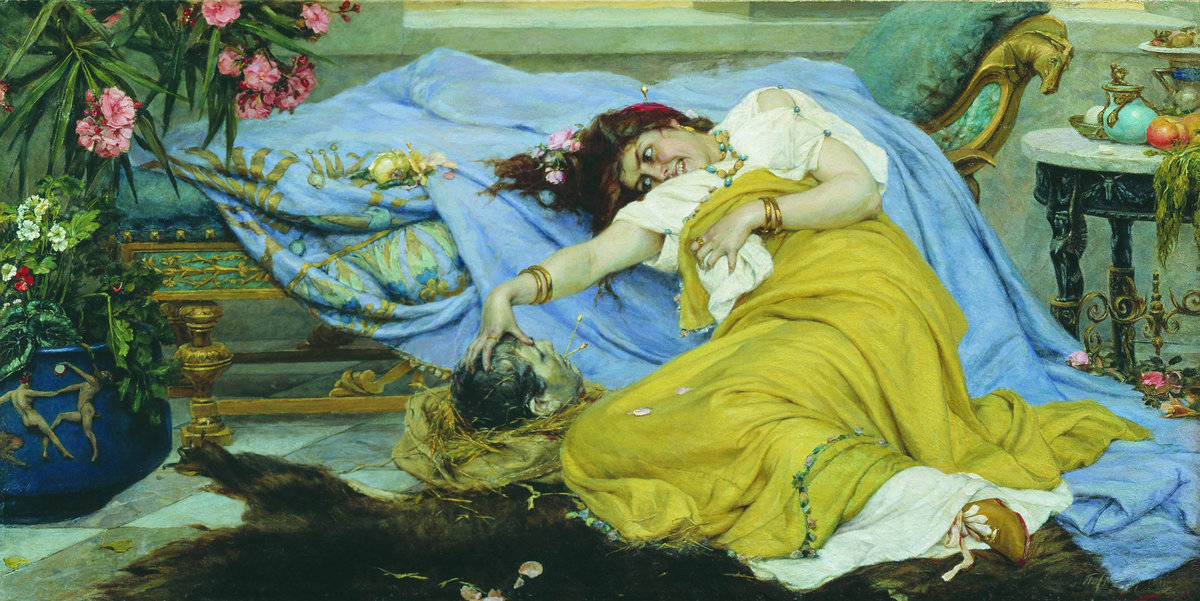
\includegraphics[scale=0.5]{holiday/159352470512026905.png}
	\label{fig:holid2} % Unique label used for referencing the figure in-text
	%\addcontentsline{toc}{figure}{Figure \ref{fig:placeholder}} % Uncomment to add the figure to the table of contents
	%	\caption{Подааарочки!!	}
\end{figure}